%% Run with the following three lines uncommented for article pdf and comment for presentation pdf
%\documentclass[a4paper]{article}
%\usepackage{beamerarticle}
%\mode<article>{\usepackage{fullpage}}
%%

%% Run with the following line uncommented for presentation pdf and commented for article pdf
\documentclass[ignorenonframetext]{beamer}
%\documentclass[ignorenonframetext,draft]{beamer}
\setbeamertemplate{navigation symbols}{}
%%

\usepackage{ esint } % for multi-dimensional integrals
\usepackage{movie15}
\usepackage{hyperref}
\usepackage{pgf}
\usepackage{subfigure}
\mode<presentation>
%{
%\usetheme{madrid}
%\usetheme{frankfurt}
	\usetheme{Copenhagen}
\useoutertheme{infolines} % this makes only immediate navigation at top of slide
%\setfootline{\insertshortinstitute, \insertshortdate
%\hfill slide \insertframenumber/\inserttotalframenumber}
%}

\title[Visualization]{Good Scientific Visualization Practices + Python}

\author{Kristen Thyng}
\date{September 19, 2013}
\institute[Texas A\&M]{ 
	Python in Geosciences}
	
% In case you want to use a logo (e.g. in png format): 
% \pgfdeclareimage[height=1.0cm]{university-logo}{figures/logo_tamu} 
% \logo{\pgfuseimage{university-logo}}

\input{../../LatexFiles/macros}

% Extra slides don't contribute to slide number at bottom right
\input{appendixnumberbeamer.sty}

\AtBeginSection[]
{
	\begin{frame}
		\frametitle{Outline}
		\tableofcontents[currentsection]
	\end{frame}
}

\begin{document}
\begin{frame}
	\titlepage
\end{frame}

\section{Overview of Bad Plotting}

% Give examples of bad plots: hard to tell what is happening, bad resolution, using the wrong kind of colormap, having a bunch of extra junk in the way. First: using the wrong kind of plot
\begin{frame}[t]\frametitle{There are lots of bad plots out there}
    
    \begin{figure}
    	\centering
    	\only<1>{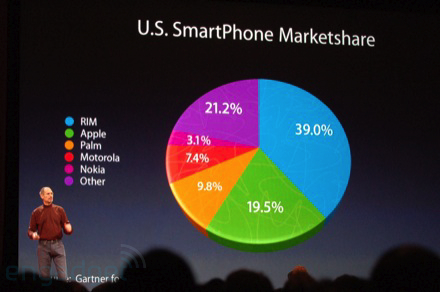
\includegraphics[width=.8\textwidth]{figures/3d}}
    	\only<2>{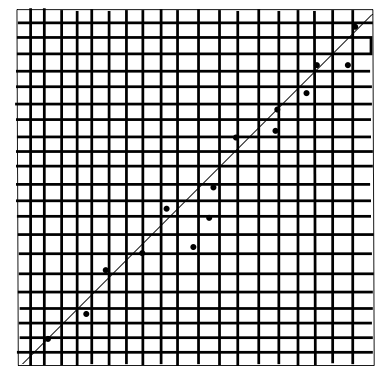
\includegraphics[width=.5\textwidth]{figures/grid}}
    	\only<3>{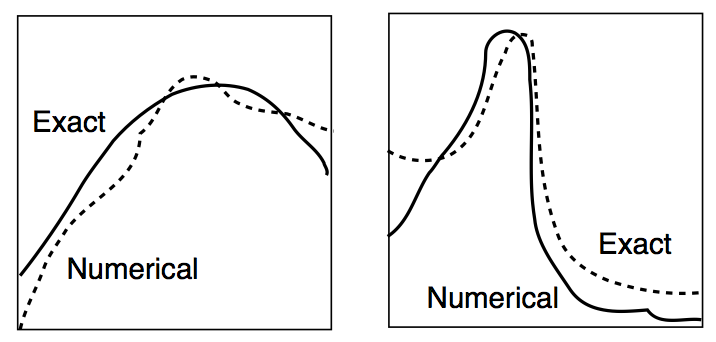
\includegraphics[width=\textwidth]{figures/consistency}}
    	\only<4>{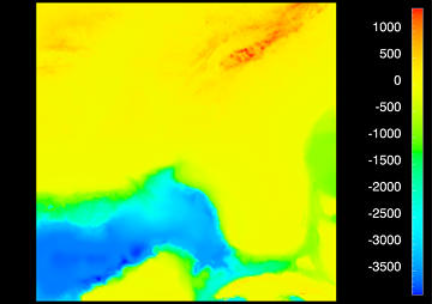
\includegraphics[width=.7\textwidth]{figures/colormap1}}
    	\only<5>{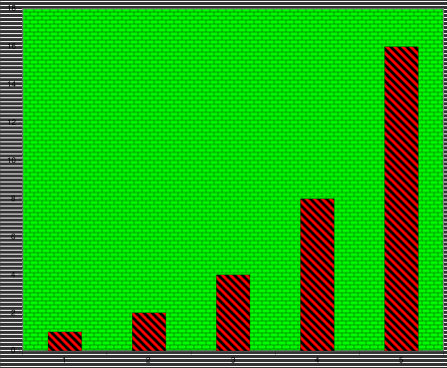
\includegraphics[width=.6\textwidth]{figures/chartjunk1}}
    \end{figure}
    \vfill
	\only<1>{Using 3D when unnecessary\\
	\tiny{http://www.engadget.com/2008/01/15/live-from-macworld-2008-steve-jobs-keynote/}}
	\only<2>{What is the dominant feature of this plot?\\
	\tiny{http://www-personal.umich.edu/~jpboyd/sciviz\_1\_graphbadly.pdf}}
	\only<3>{Inconsistent representations\\
	\tiny{http://www-personal.umich.edu/~jpboyd/sciviz\_1\_graphbadly.pdf}}
	\only<4>{Unintuitive representation\\
	\tiny{http://www.research.ibm.com/people/l/lloydt/color/color.HTM}}
	\only<5>{Chart junk\\
	\tiny{http://en.wikipedia.org/wiki/File:Chartjunk-example.svg, Tufte, Edward R. (1983). The Visual Display of Quantitative Information. Cheshire, CT: Graphics Press.}}

\end{frame}


\begin{frame}[t]\frametitle{Goals in Visualization}
    \huge{
	\begin{itemize}
		\item Honestly present the information - no cheating!
		\item Clear presentation - nothing unnecessary
		\item Label axes, units, etc, with large lettering
		\item Intuitive, consistent markers/coloring
		\item Give context
	\end{itemize}}
\end{frame}


\begin{frame}[t]\frametitle{Better plots}
    \vskip-2ex
    \begin{figure}
    	\centering
    	\only<1>{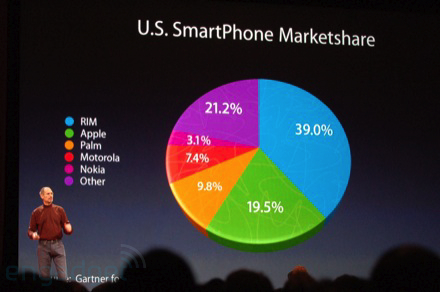
\includegraphics[width=.8\textwidth]{figures/3d}}
    	\only<2>{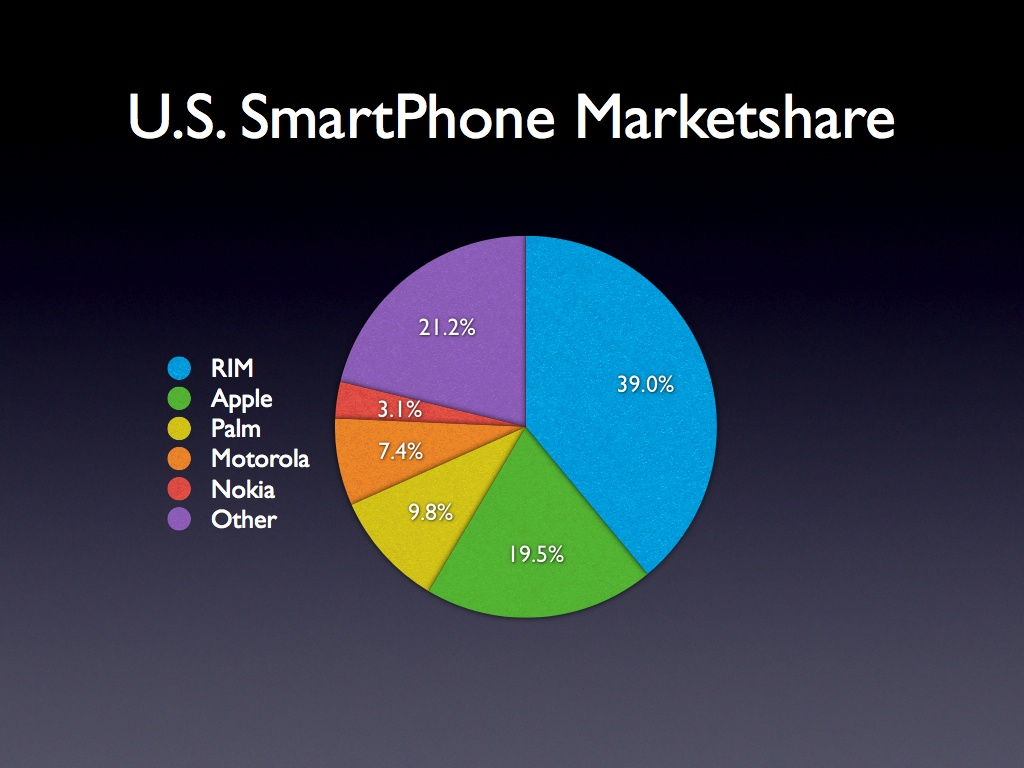
\includegraphics[width=.7\textwidth]{figures/3dfixed}}
    	\only<3>{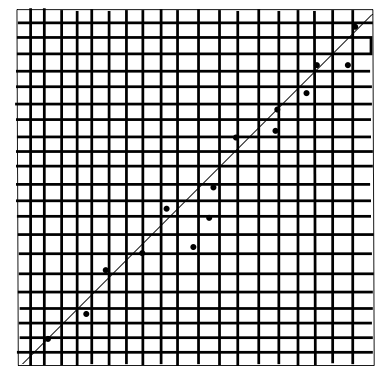
\includegraphics[width=.5\textwidth]{figures/grid}}
    	\only<4>{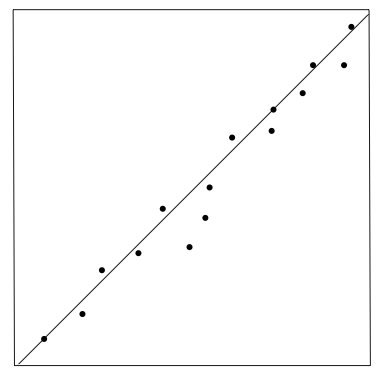
\includegraphics[width=.5\textwidth]{figures/gridfixed}}
    	\only<5>{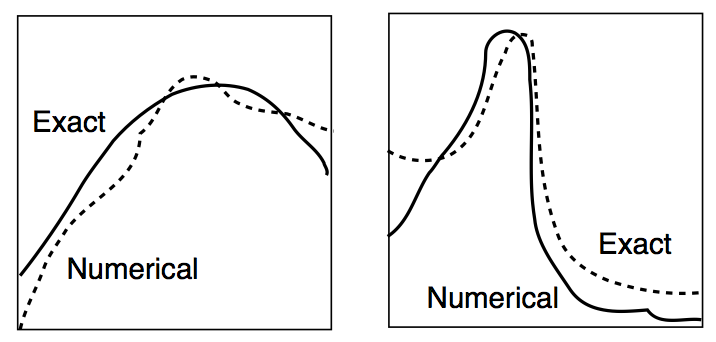
\includegraphics[width=\textwidth]{figures/consistency}}
    	\only<6>{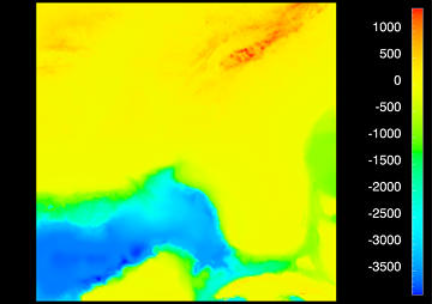
\includegraphics[width=.7\textwidth]{figures/colormap1}}
    	\only<7>{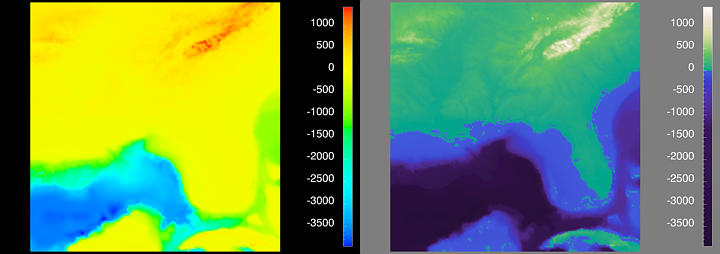
\includegraphics[width=\textwidth]{figures/colormap}}
    	\only<8>{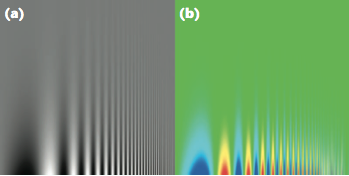
\includegraphics[width=.8\textwidth]{figures/colormap_example}}
    	\only<9>{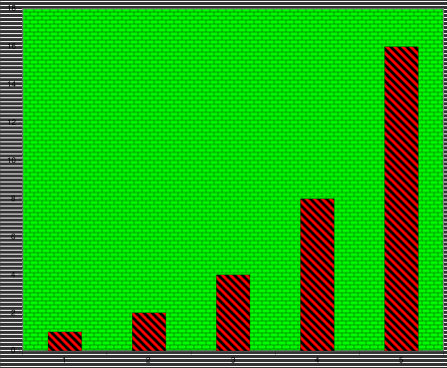
\includegraphics[width=.6\textwidth]{figures/chartjunk1}}
    \end{figure}
	\only<1>{Using 3D when unnecessary\\
	\tiny{http://www.engadget.com/2008/01/15/live-from-macworld-2008-steve-jobs-keynote/}}
	\only<2>{Better presentation, though pie charts not great\\
	\tiny{http://www.quora.com/Data-Visualization/What-should-everyone-know-about-making-good-charts-and-graphs-to-represent-data}}
	\only<3>{What is the dominant feature of this plot?\\
	\tiny{http://www-personal.umich.edu/~jpboyd/sciviz\_1\_graphbadly.pdf}}
	\only<4>{Simpler is often better\\
	\tiny{http://www-personal.umich.edu/~jpboyd/sciviz\_1\_graphbadly.pdf}}
	\only<5>{Pick a representation and stick with it\\
	\tiny{http://www-personal.umich.edu/~jpboyd/sciviz\_1\_graphbadly.pdf}}
	\only<6>{Unintuitive representation\\
	\tiny{http://www.research.ibm.com/people/l/lloydt/color/color.HTM}}
	\only<7>{\vfill Color choices are key\\
	\tiny{http://www.research.ibm.com/people/l/lloydt/color/color.HTM}}
	\only<8>{\vfill Color choices are key\\
	\tiny{http://www.sv.vt.edu/~rkriz/Projects/create\_color\_table/color\_07.pdf}}
	\only<9>{Chart junk\\
	\tiny{http://en.wikipedia.org/wiki/File:Chartjunk-example.svg, Tufte, Edward R. (1983). The Visual Display of Quantitative Information. Cheshire, CT: Graphics Press.}}

\end{frame}


%%% Colors, Specifically %%%
\section{Perceptually-based colormaps}


% Explain stuff as in IBM article, with reference
\begin{frame}[t]\frametitle{Data Types}
    \begin{columns}
    \begin{column}{5cm}
	\begin{itemize}
	\only<1>{
		\item Categorical: Representing discrete things, not on continuum
		\item Interval or sequential: intervals of the data are equal distances
		\item Ratio or diverging: has critical value (often 0) and ratios of values are equal}
	\only<2>{
		\item {\bf \color{red}{Categorical: Representing discrete things, not on continuum}}
		\item Interval or sequential: intervals of the data are equal distances
		\item Ratio or diverging: has critical value (often 0) and ratios of values are equal}
	\only<3>{
		\item Categorical: Representing discrete things, not on continuum
		\item {\bf \color{blue}{Interval or sequential: intervals of the data are equal distances}}
		\item Ratio or diverging: has critical value (often 0) and ratios of values are equal}
	\only<4,5>{
		\item Categorical: Representing discrete things, not on continuum
		\item Interval or sequential: intervals of the data are equal distances
		\item {\bf \color{brown}{Ratio or diverging: has critical value (often 0) and ratios of values are equal}}}
	\only<6>{
		\item Categorical: Representing discrete things, not on continuum
		\item {\bf Interval or sequential: intervals of the data are equal distances}
		\item {\bf Ratio or diverging: has critical value (often 0) and ratios of values are equal}}
	\end{itemize}
	\only<6>{$\Rightarrow$ Equal steps in data should correspond to equal steps in perception}
	\vfill
	\end{column}
    \begin{column}{7cm}
	\begin{figure}
		\centering
		\only<1,2>{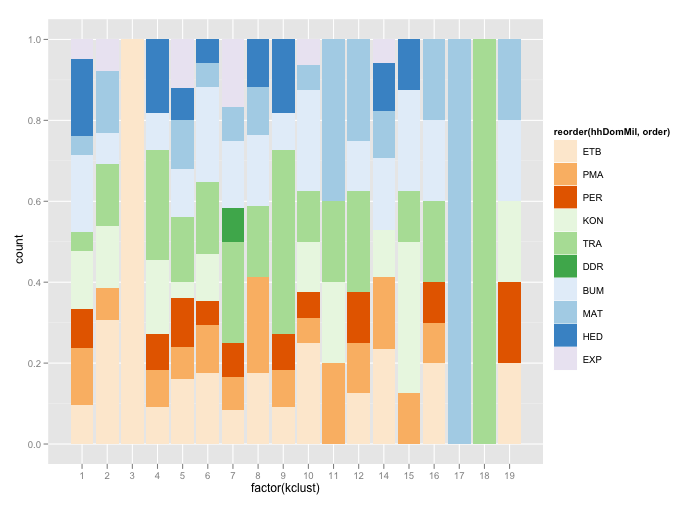
\includegraphics[width=\textwidth]{figures/categorical}}
		\only<3>{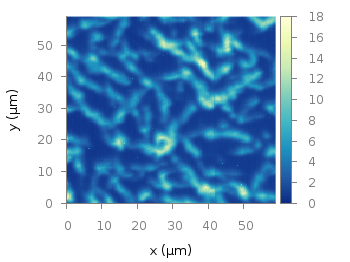
\includegraphics[width=\textwidth]{figures/sequential}}
		\only<4>{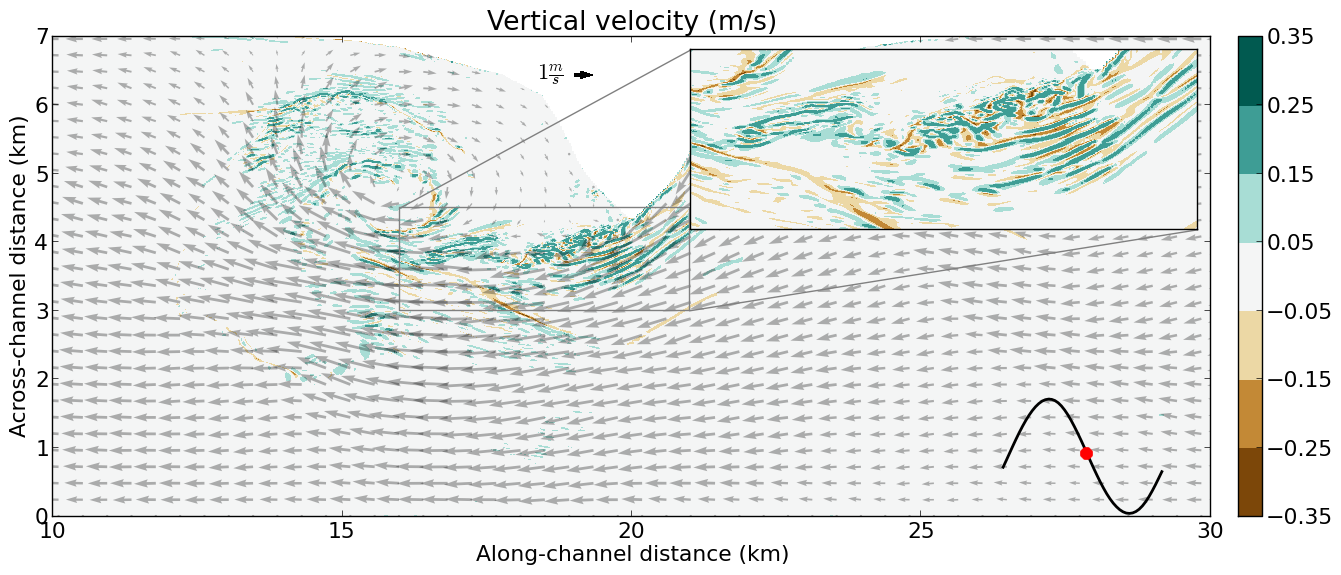
\includegraphics[width=\textwidth]{figures/w26inset}}
		\only<5,6>{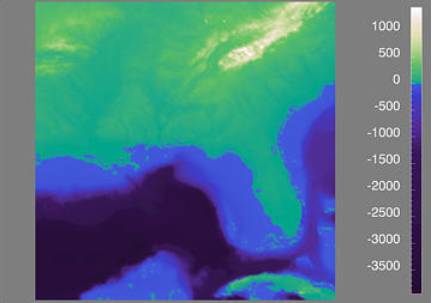
\includegraphics[width=\textwidth]{figures/colormap2}}
	\end{figure}
	\only<1,2>{\tiny{http://stackoverflow.com/questions/7150453/order-categorical-data-in-a-stacked-bar-plot-with-ggplot2}}
	\only<3>{\tiny{http://www.gnuplotting.org/tag/colormap/}}
	\end{column}
	\end{columns}
	\vfill
    \tiny{http://www.research.ibm.com/people/l/lloydt/color/color.HTM}
\end{frame}


% Human Perception: IBM stuff and lightness, and what it tells us about colormaps
\begin{frame}[t]\frametitle{Color is 3D}
    \begin{figure}
    	\centering
    	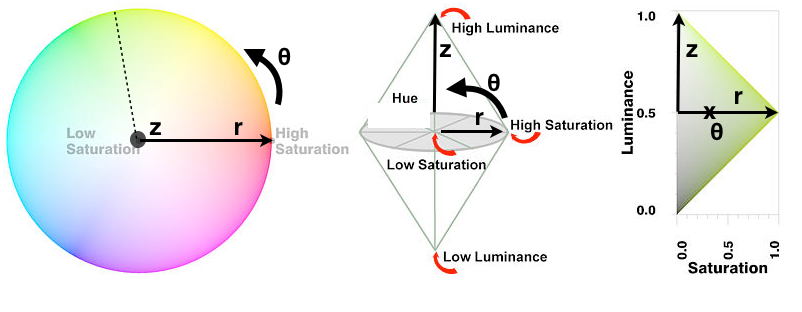
\includegraphics[width=\textwidth]{figures/color3d}
    \end{figure}
    \only<1>{$r$: saturation/color intensity, $z$: luminance/brightness, $\theta$: color hue}
    \only<2>{{\bf\color{red}$r$: saturation/color intensity, $z$: luminance/brightness}, $\theta$: color hue\\
    {\color{red}$\Rightarrow$ good for representing continuous variations in data magnitude}}
    \tiny{http://www.research.ibm.com/people/l/lloydt/color/color.HTM}
\end{frame}


% Jet luminance
\begin{frame}[t]\frametitle{Jet Luminance}
    \begin{figure}
    	\centering
    	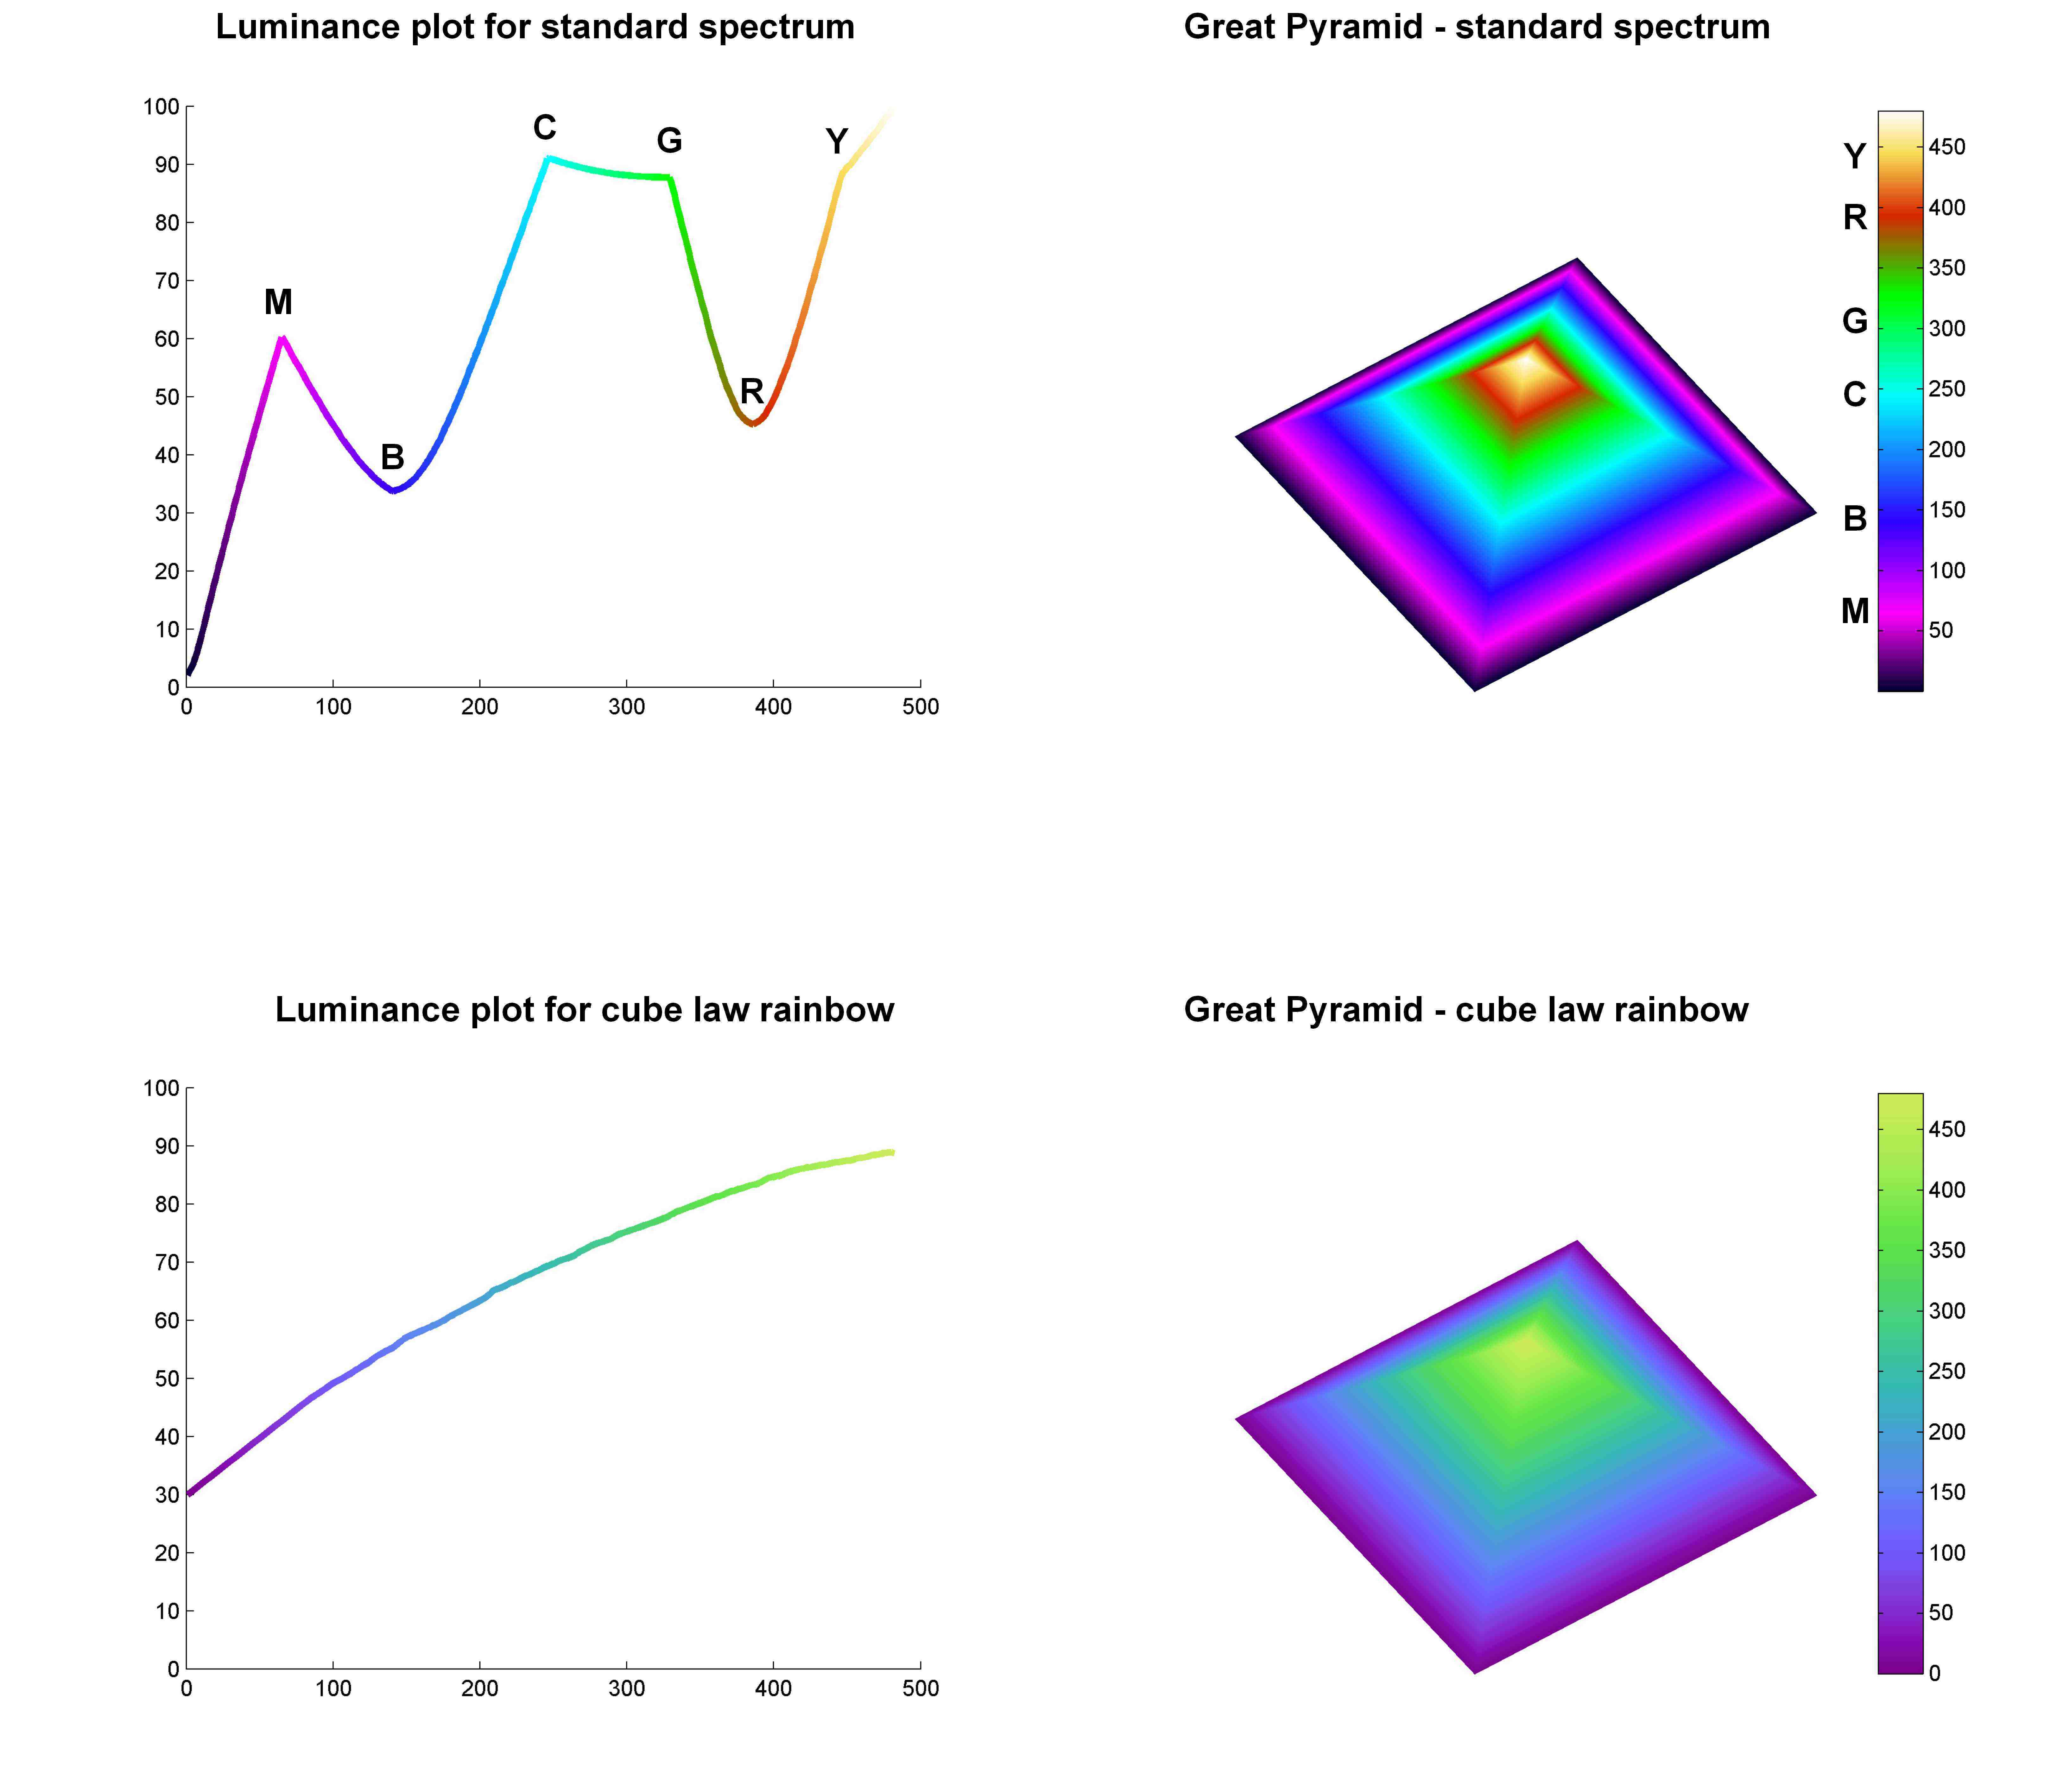
\includegraphics[width=.6\textwidth]{figures/jet_luminance.jpg}
    \end{figure}
    \tiny{http://www.mathworks.com/matlabcentral/fx\_files/28982/16/spectrum\_vs\_cubicYF.png}
\end{frame}


% Show IBM colormap comparison
\begin{frame}[t]\frametitle{Hue-based Colormaps Perceptually Distort Information}
    \begin{figure}
    	\centering
    	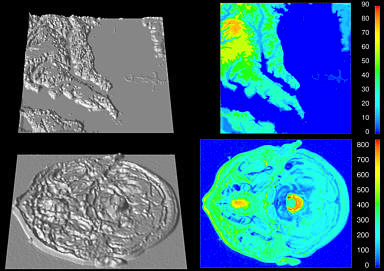
\includegraphics[width=.475\textwidth]{figures/bw_vs_jet1}
    	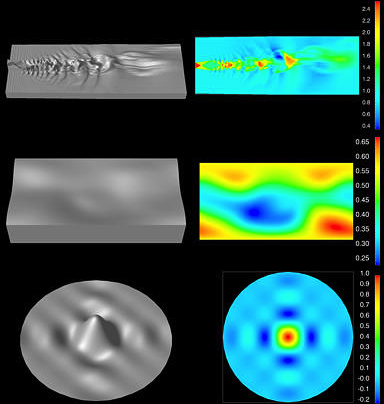
\includegraphics[width=.475\textwidth]{figures/bw_vs_jet2}
    \end{figure}
    \tiny{http://www.research.ibm.com/people/l/lloydt/color/color.HTM}
\end{frame}


% Show IBM luminance and saturation comparison
\begin{frame}[t]\frametitle{Luminance and Saturation Colormaps}
    \begin{figure}
    	\centering
    	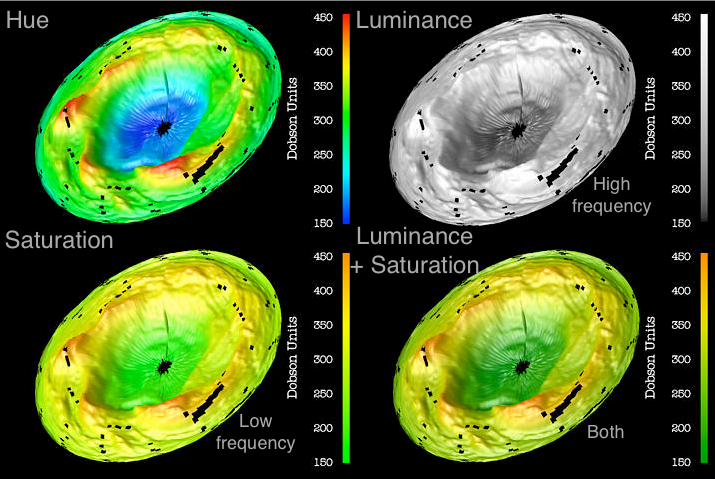
\includegraphics[width=.8\textwidth]{figures/luminance_vs_saturation.png}
    \end{figure}
    \tiny{http://www.research.ibm.com/people/l/lloydt/color/color.HTM}
\end{frame}


% More IBM examples
\begin{frame}[t]\frametitle{Improved Colormapping}
	\vskip-2ex
    \begin{figure}
    	\centering
    	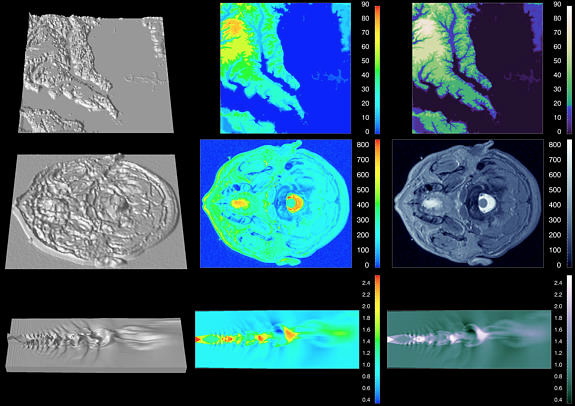
\includegraphics[width=.8\textwidth]{figures/maps_together}
    \end{figure}
    \tiny{http://www.research.ibm.com/people/l/lloydt/color/color.HTM}
\end{frame}



\section{Matplotlib Tools}


% Explain colormap types and show matplotlib gallery.
\begin{frame}[t]\frametitle{Types of Colormaps}
	\begin{figure}
		\centering
		\only<1>{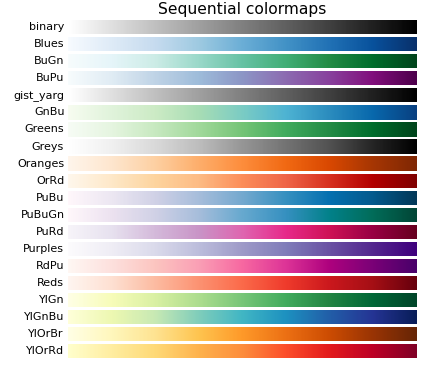
\includegraphics[width=.7\textwidth]{figures/colormaps_sequential}}
		\only<2>{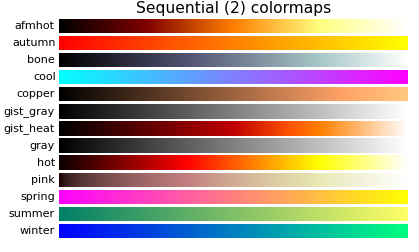
\includegraphics[width=.7\textwidth]{figures/colormaps_sequential2}}
		\only<3>{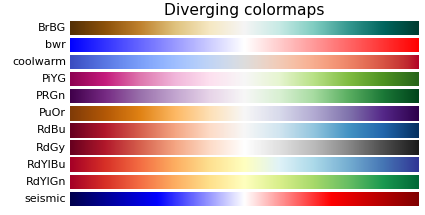
\includegraphics[width=.7\textwidth]{figures/colormaps_diverging}}
		\only<4>{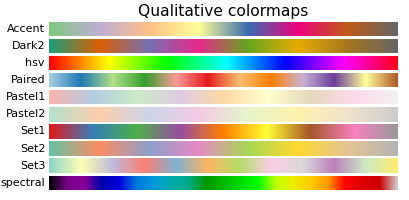
\includegraphics[width=.7\textwidth]{figures/colormaps_qualitative}}
		\only<5>{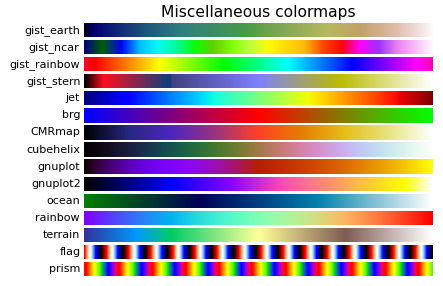
\includegraphics[width=.7\textwidth]{figures/colormaps_misc}}
	\end{figure}
	\vfill
	\tiny{http://matplotlib.org/examples/color/colormaps\_reference.html}
\end{frame}



% Show tools in Matplotlib to do good things: subplot, axesgrid (?), controlling your actual axes. I have some of my own examples of these from the EWTEC paper.
\begin{frame}[t]\frametitle{Subplot}
	\begin{figure}
		\centering
		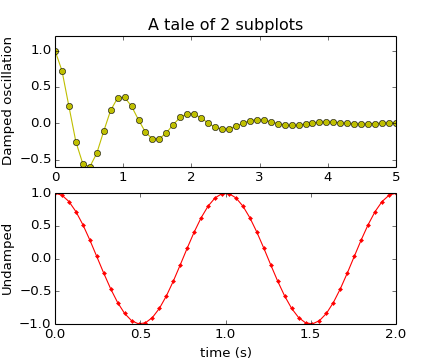
\includegraphics[width=.6\textwidth]{figures/subplot_demo2}
	\end{figure}
	\tiny{http://matplotlib.org/examples/subplots\_axes\_and\_figures/subplot\_demo.html}
\end{frame}


\begin{frame}[t]\frametitle{Axes Grid Toolbox}
	\begin{figure}
		\centering
		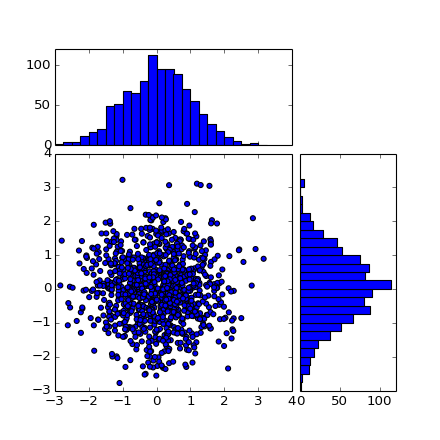
\includegraphics[width=.6\textwidth]{figures/axes_grid}
	\end{figure}
	\tiny{http://matplotlib.org/examples/axes\_grid/scatter\_hist.html}
\end{frame}


\begin{frame}[t]\frametitle{Inset Axes}
	\begin{figure}
		\centering
		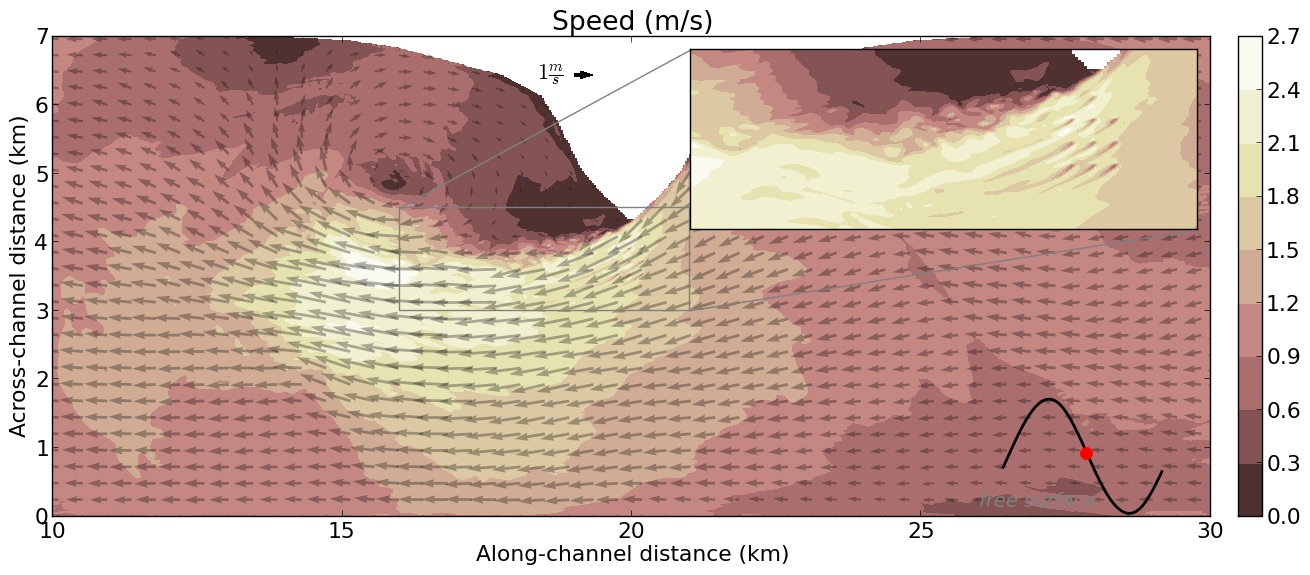
\includegraphics[width=\textwidth]{figures/s26inset}
	\end{figure}
\end{frame}


\begin{frame}[t]\frametitle{Overlaid Axes}
	\begin{figure}
		\centering
		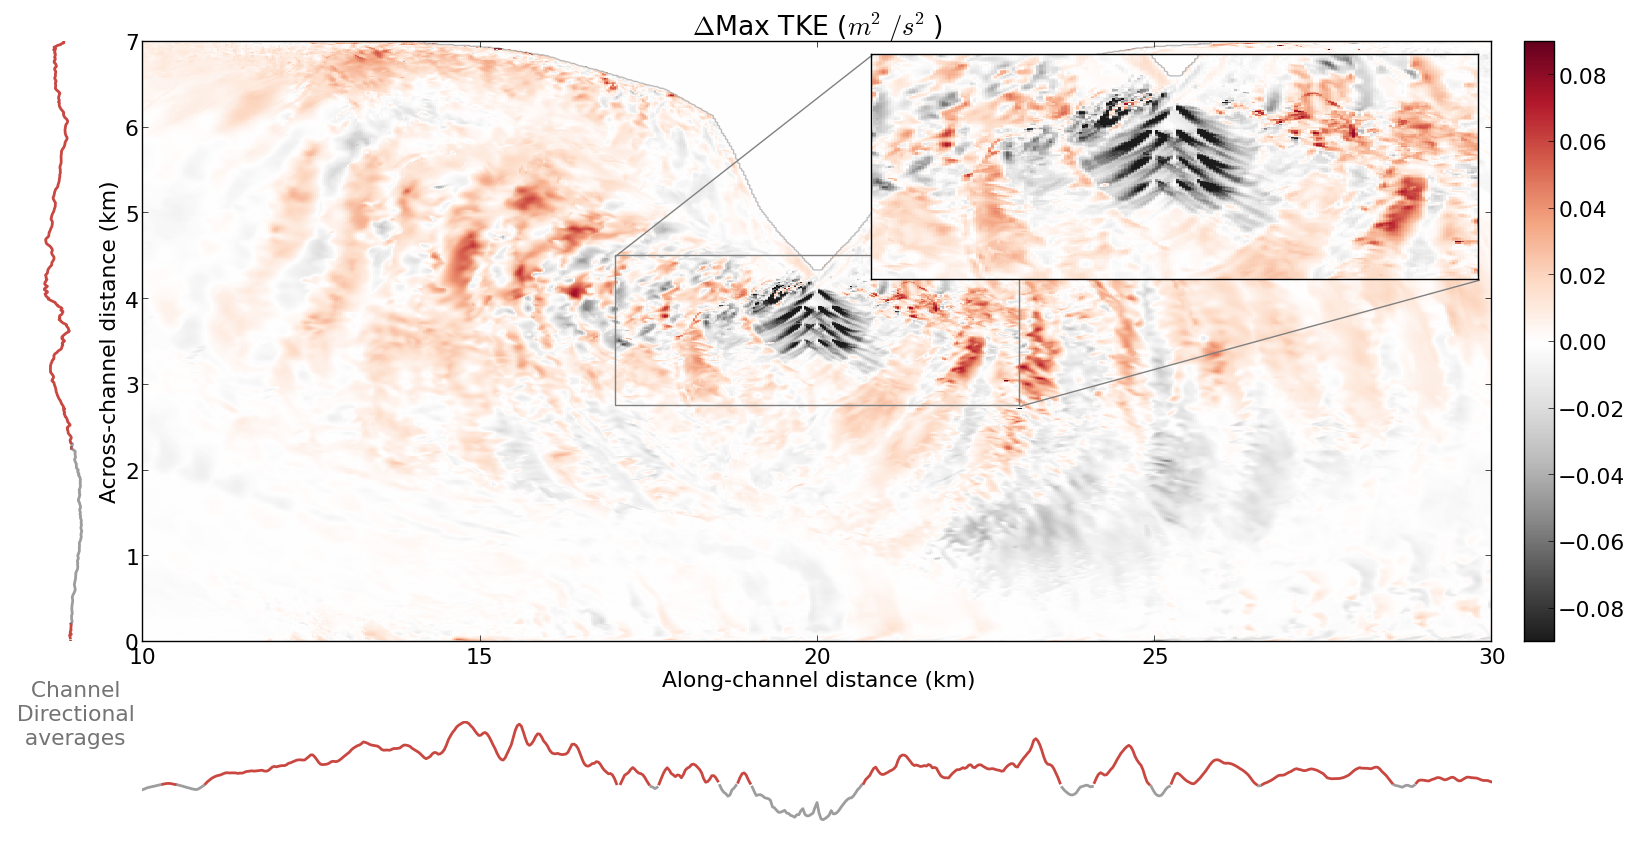
\includegraphics[width=\textwidth]{figures/tkemax}
	\end{figure}
\end{frame}


\begin{frame}[t]\frametitle{Overlaid Axes: Colorbar Placement}
	\begin{figure}
		\centering
		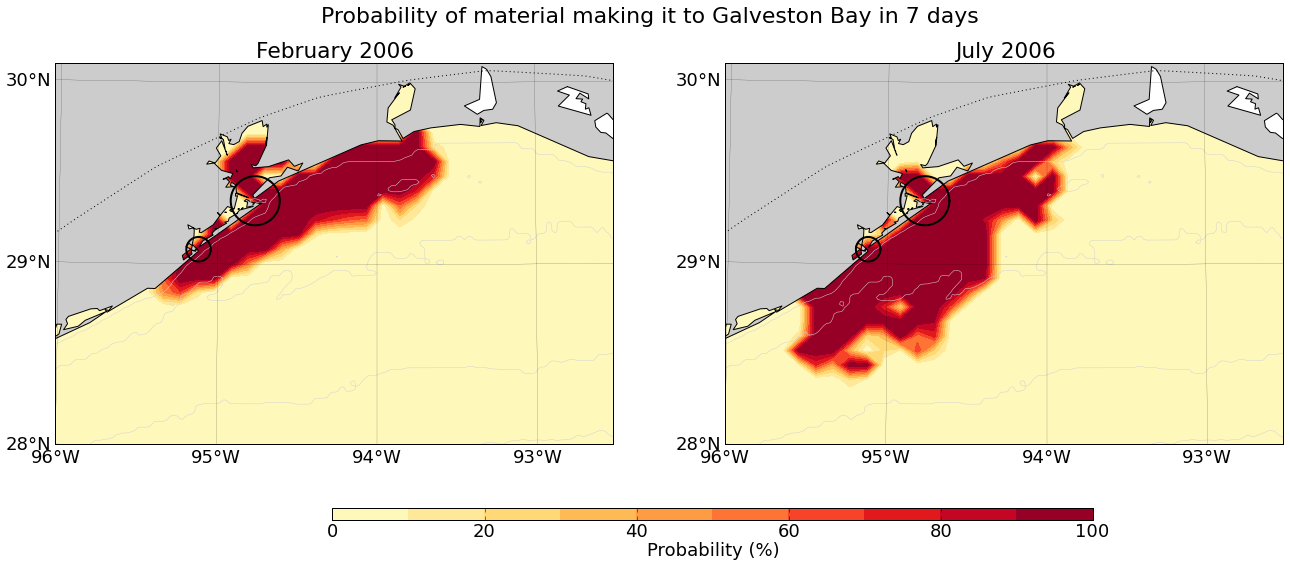
\includegraphics[width=\textwidth]{figures/galvestonzoomhistcontour}
	\end{figure}
\end{frame}



\section{Miscellaneous Considerations}


% More IBM examples
\begin{frame}[t]\frametitle{Use Colormaps for Different Purposes}
    \begin{figure}
    	\centering
    	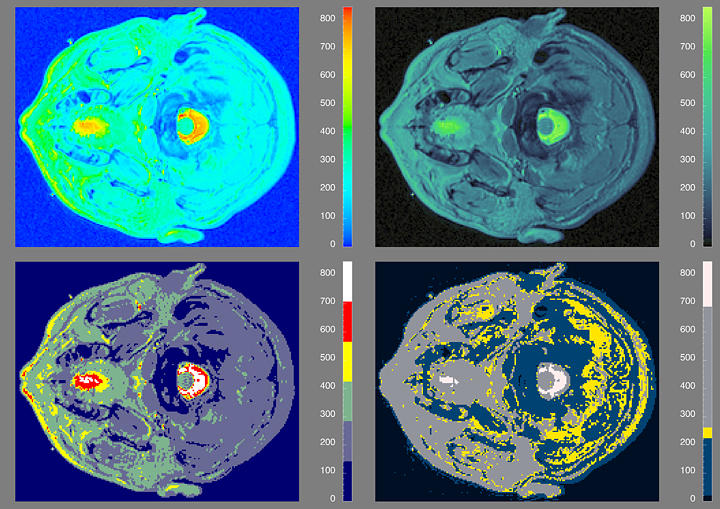
\includegraphics[width=.75\textwidth]{figures/multiple_colormaps}
    \end{figure}
    \tiny{http://www.research.ibm.com/people/l/lloydt/color/color.HTM}
\end{frame}


% Want to use human perception for presentation, but also intuition and pattern
% Cube Helix
\begin{frame}[t]\frametitle{Cube Helix}
    \begin{figure}
    	\centering
    	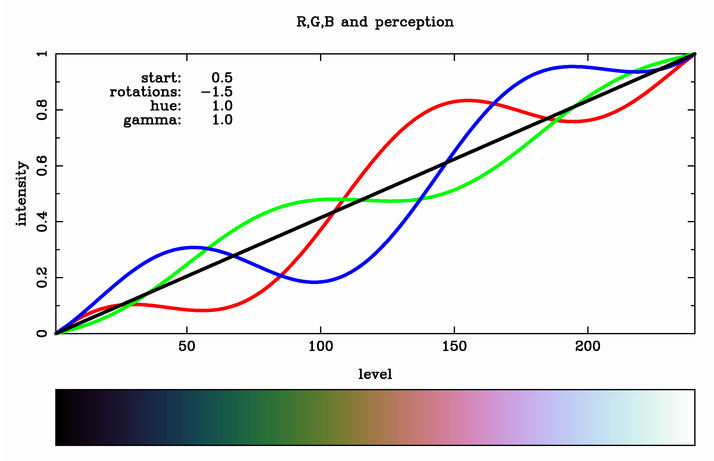
\includegraphics[width=.7\textwidth]{figures/cube_helix}
    \end{figure}
    Proper intensity scaling, though do consider application
    \tiny{http://www.mrao.cam.ac.uk/~dag/CUBEHELIX/}
\end{frame}


% Give context
\begin{frame}[t]\frametitle{Give Context}
	\begin{figure}
		\centering
		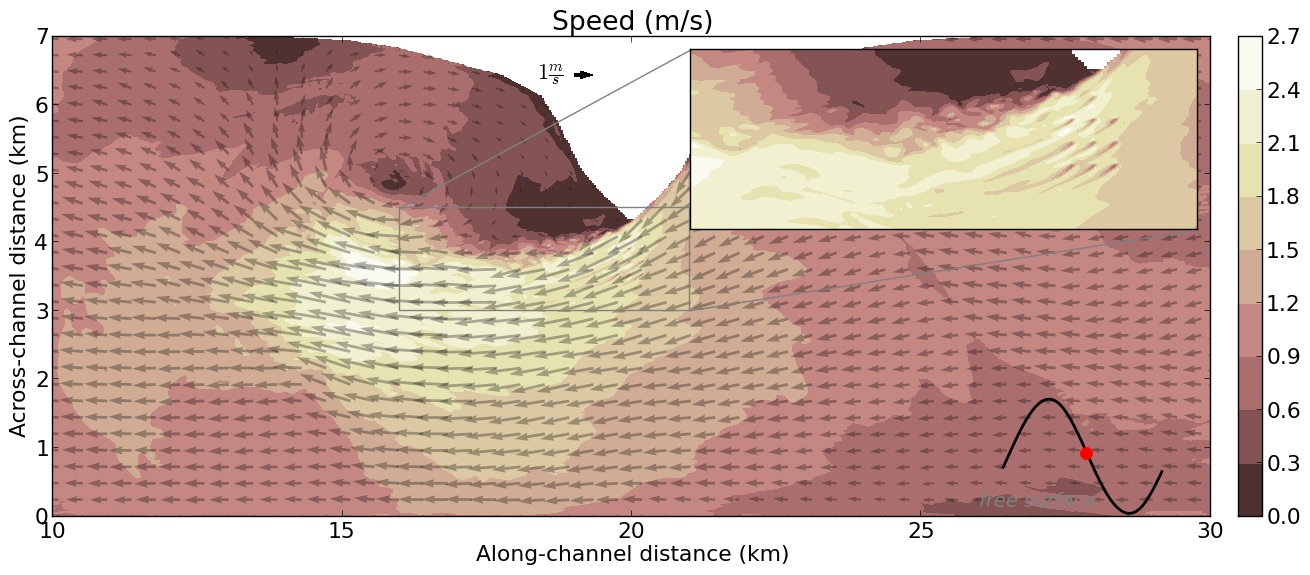
\includegraphics[width=\textwidth]{figures/s26inset}
	\end{figure}
\end{frame}


% Choose an colormap for a variable and stick with it. Show kinds of vertical velocity plots of mine.
\begin{frame}[t]\frametitle{Be Consistent}
	\vskip-2ex
	\begin{figure}
		\centering
		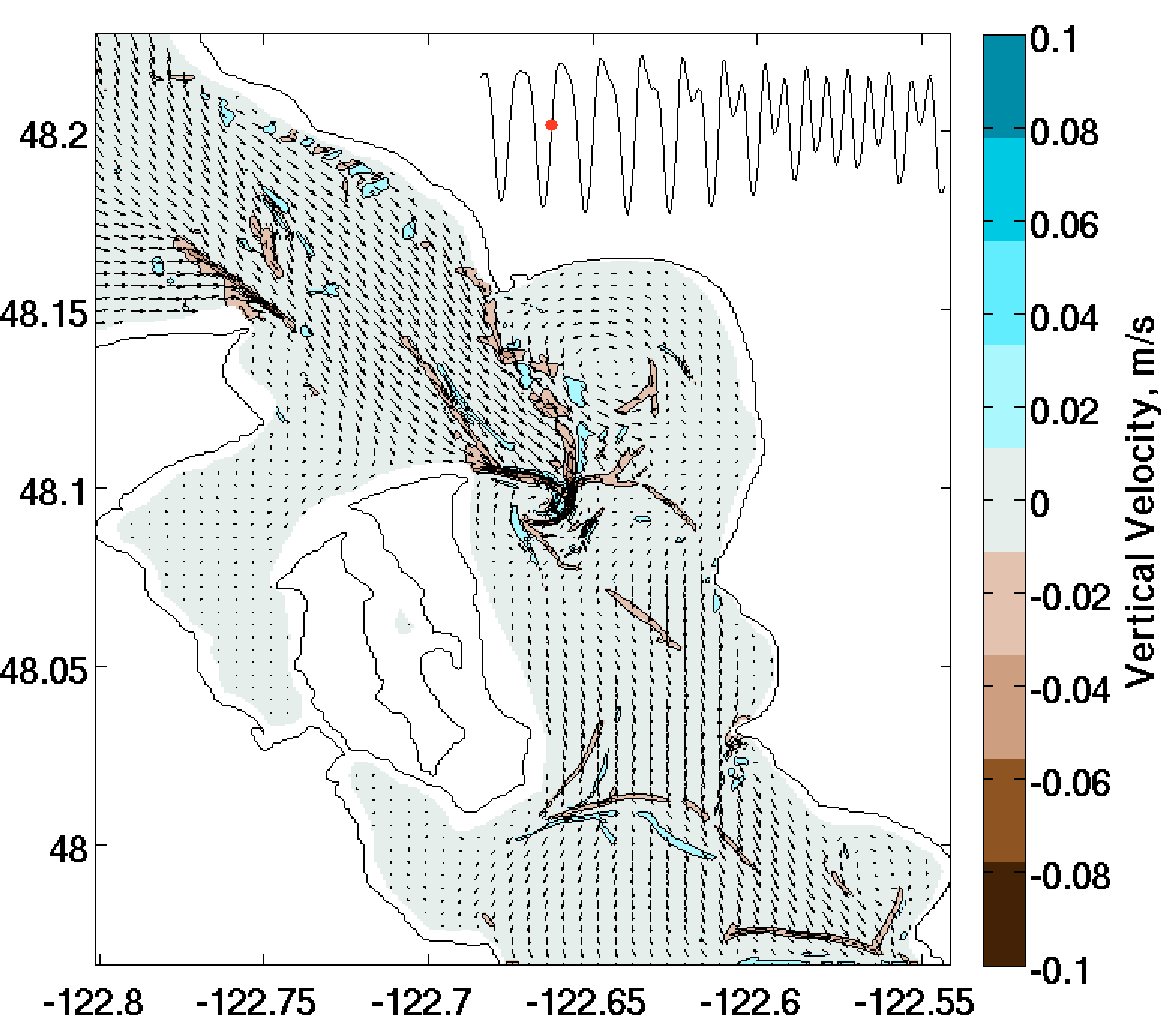
\includegraphics[width=.37\textwidth]{figures/w171}
		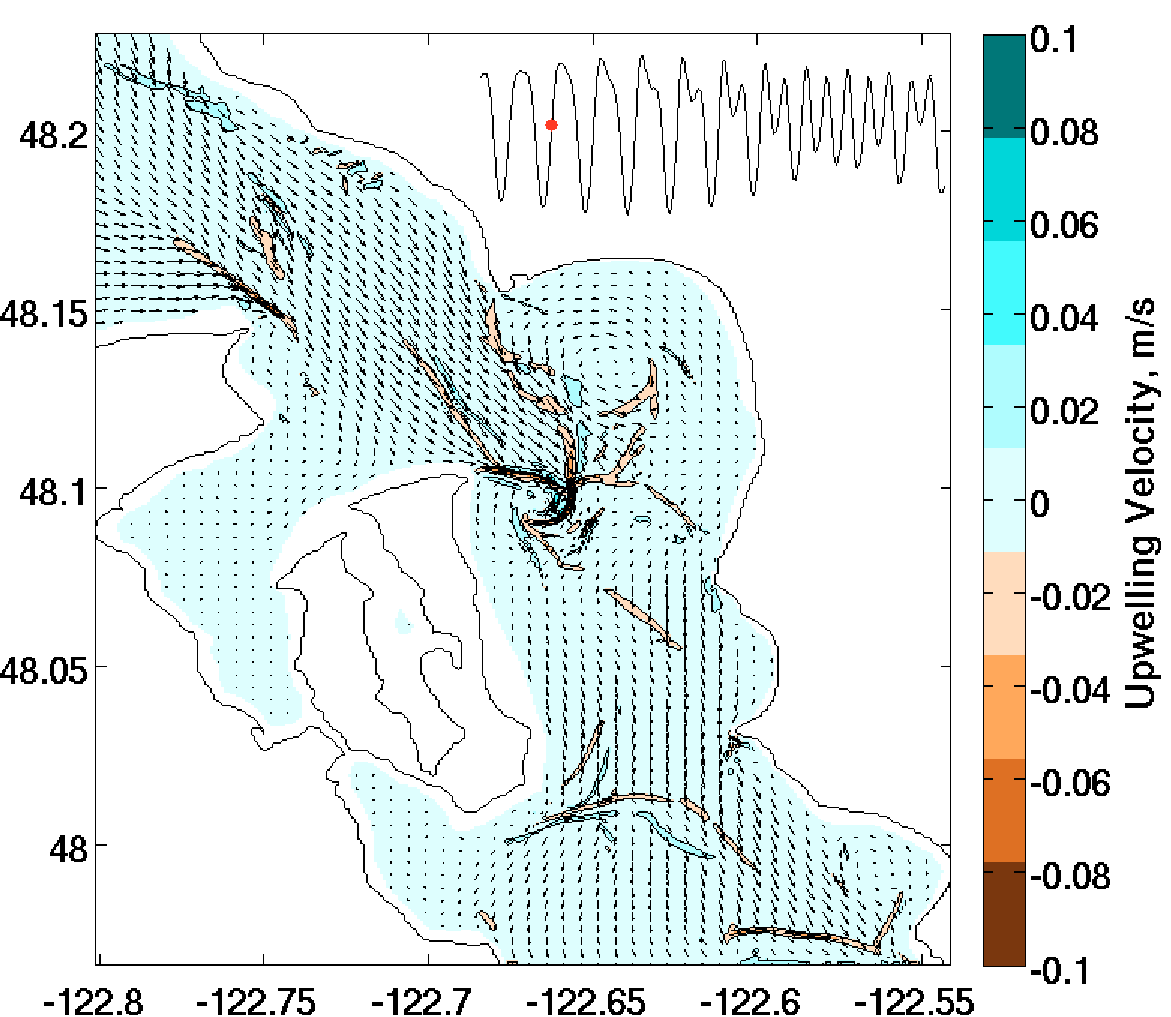
\includegraphics[width=.37\textwidth]{figures/wuw171}\\
		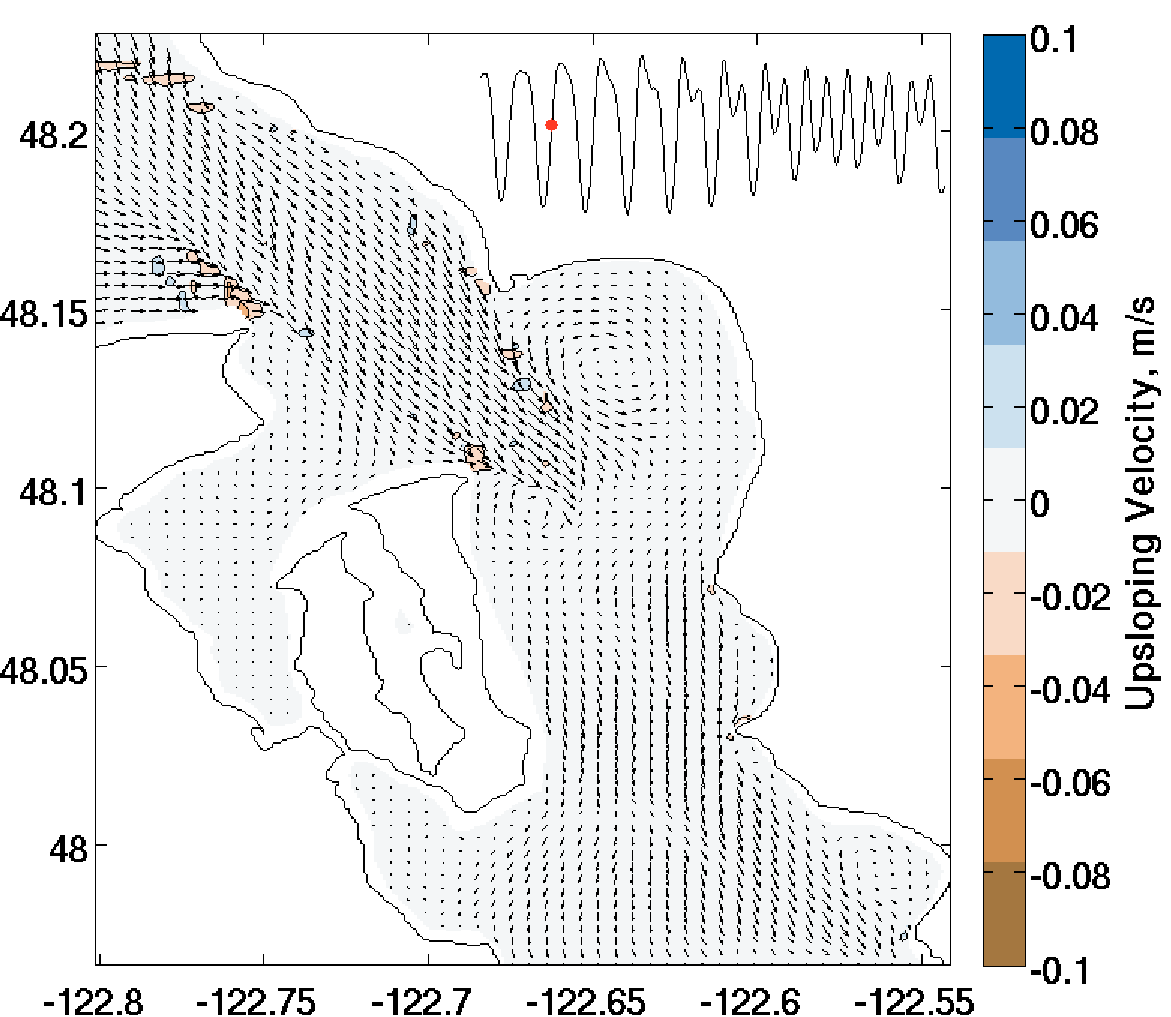
\includegraphics[width=.37\textwidth]{figures/wus171}
	\end{figure}
\end{frame}


% Discrete vs. Continuous colorbar (maybe use Admiralty Inlet topo/bathy plot, and Sally's)
\begin{frame}[t]\frametitle{Discrete vs. Continuous Colorbar}
	\begin{figure}
		\centering
		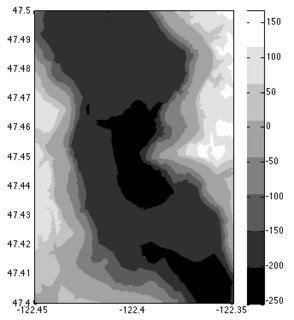
\includegraphics[width=.45\textwidth]{figures/bathy_discrete}
		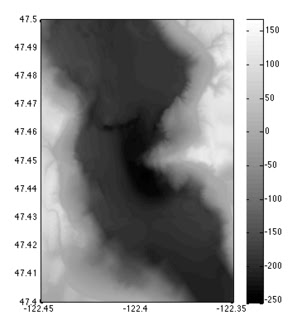
\includegraphics[width=.45\textwidth]{figures/bathy_continuous}
	\end{figure}
    \tiny{http://figuredesign.blogspot.com/2012/04/meeting-recap-colors-in-figures.html}
\end{frame}



% Diverging colormap: around zero, white or not? (vorticity), maybe use a line like Eleanor
\begin{frame}[t]\frametitle{Diverging Colormap: Critical value treatment}
	\begin{figure}
		\centering
		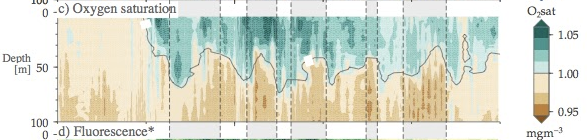
\includegraphics[width=.9\textwidth]{figures/critical_line}\\
		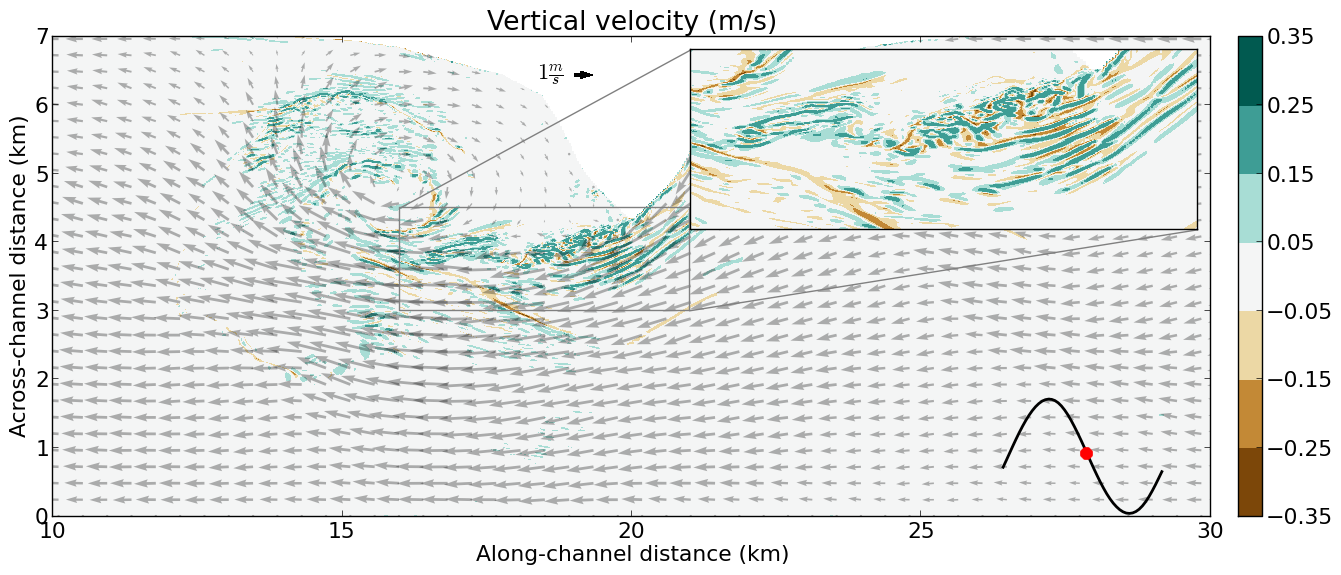
\includegraphics[width=.8\textwidth]{figures/w26inset}
	\end{figure}
    \tiny{http://figuredesign.blogspot.com/2012/04/meeting-recap-colors-in-figures.html}
\end{frame}



% Printing in black and white from color
\begin{frame}[t]\frametitle{Printing in Black and White from Color}
	\vskip-2ex
	\begin{figure}
		\centering
		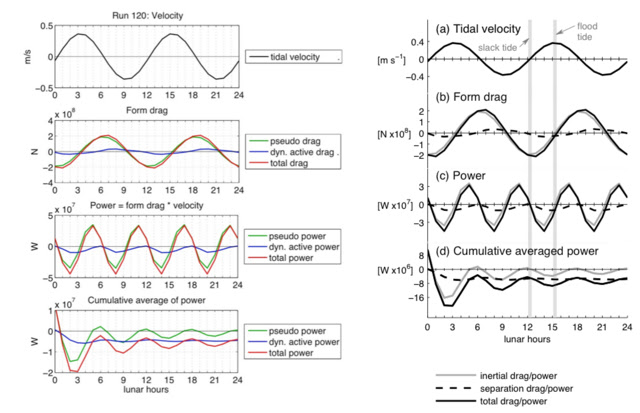
\includegraphics[width=.75\textwidth]{figures/bw_color_line_plot}
	\end{figure}
	Change the design choices altogether, or be sure the colors will print to different grayscale values\\
    \tiny{http://figuredesign.blogspot.com/2012/04/meeting-recap-colors-in-figures.html}
\end{frame}



% Show colorblind website and example output from it
\begin{frame}[t]\frametitle{Color Blindness}
	\begin{figure}
		\centering
		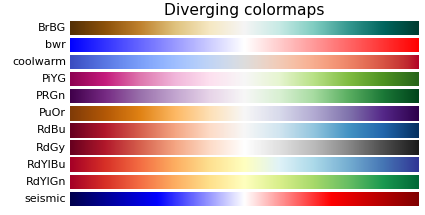
\includegraphics[width=.45\textwidth]{figures/colormaps_diverging}
		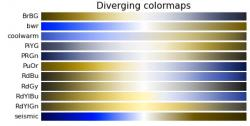
\includegraphics[width=.45\textwidth]{figures/colormaps_diverging_deuteranopia}\\
		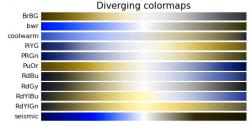
\includegraphics[width=.45\textwidth]{figures/colormaps_diverging_protanopia}
		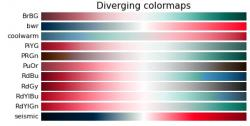
\includegraphics[width=.45\textwidth]{figures/colormaps_diverging_tritanopia}
	\end{figure}
	Problems distinguishing green-yellow-red, and rarely blue-yellow
	\tiny{http://www.etre.com/tools/colourblindsimulator/}
\end{frame}


% Resources
\begin{frame}[t]\frametitle{Resources}
	\vskip-2ex
    \begin{itemize}
    	\item Edward Tufte's books
    	\item IBM articles: http://www.research.ibm.com/people/l/lloydt/color/color.HTM
    	\item Color Brewer: Color advice for maps: http://colorbrewer2.org
    	\item IEEE Computer Society article: http://www.sv.vt.edu/~rkriz/Projects/create\_color\_table/color\_07.pdf
    	\item MatLab colormap function, with lots of references: http://www.mathworks.com/matlabcentral/fileexchange/28982-perceptually-improved-colormaps/content/pmkmp.m
    	\item Cube Helix colormap: http://www.mrao.cam.ac.uk/~dag/CUBEHELIX/
    	\item Test plots for sensitivity to color blindness: http://www.etre.com/tools/colourblindsimulator/
    	\item Matplotlib example gallery: http://matplotlib.org/gallery.html
    	\item Useful design blog: http://figuredesign.blogspot.com
    	\item Figures writeup: http://www-personal.umich.edu/~jpboyd/sciviz\_1\_graphbadly.pdf
    \end{itemize}
\end{frame}


\end{document}